\documentclass[twoside]{book}

% Packages required by doxygen
\usepackage{fixltx2e}
\usepackage{calc}
\usepackage{doxygen}
\usepackage[export]{adjustbox} % also loads graphicx
\usepackage{graphicx}
\usepackage[utf8]{inputenc}
\usepackage{makeidx}
\usepackage{multicol}
\usepackage{multirow}
\PassOptionsToPackage{warn}{textcomp}
\usepackage{textcomp}
\usepackage[nointegrals]{wasysym}
\usepackage[table]{xcolor}

% Font selection
\usepackage[T1]{fontenc}
\usepackage[scaled=.90]{helvet}
\usepackage{courier}
\usepackage{amssymb}
\usepackage{sectsty}
\renewcommand{\familydefault}{\sfdefault}
\allsectionsfont{%
  \fontseries{bc}\selectfont%
  \color{darkgray}%
}
\renewcommand{\DoxyLabelFont}{%
  \fontseries{bc}\selectfont%
  \color{darkgray}%
}
\newcommand{\+}{\discretionary{\mbox{\scriptsize$\hookleftarrow$}}{}{}}

% Page & text layout
\usepackage{geometry}
\geometry{%
  a4paper,%
  top=2.5cm,%
  bottom=2.5cm,%
  left=2.5cm,%
  right=2.5cm%
}
\tolerance=750
\hfuzz=15pt
\hbadness=750
\setlength{\emergencystretch}{15pt}
\setlength{\parindent}{0cm}
\setlength{\parskip}{3ex plus 2ex minus 2ex}
\makeatletter
\renewcommand{\paragraph}{%
  \@startsection{paragraph}{4}{0ex}{-1.0ex}{1.0ex}{%
    \normalfont\normalsize\bfseries\SS@parafont%
  }%
}
\renewcommand{\subparagraph}{%
  \@startsection{subparagraph}{5}{0ex}{-1.0ex}{1.0ex}{%
    \normalfont\normalsize\bfseries\SS@subparafont%
  }%
}
\makeatother

% Headers & footers
\usepackage{fancyhdr}
\pagestyle{fancyplain}
\fancyhead[LE]{\fancyplain{}{\bfseries\thepage}}
\fancyhead[CE]{\fancyplain{}{}}
\fancyhead[RE]{\fancyplain{}{\bfseries\leftmark}}
\fancyhead[LO]{\fancyplain{}{\bfseries\rightmark}}
\fancyhead[CO]{\fancyplain{}{}}
\fancyhead[RO]{\fancyplain{}{\bfseries\thepage}}
\fancyfoot[LE]{\fancyplain{}{}}
\fancyfoot[CE]{\fancyplain{}{}}
\fancyfoot[RE]{\fancyplain{}{\bfseries\scriptsize Generated by Doxygen }}
\fancyfoot[LO]{\fancyplain{}{\bfseries\scriptsize Generated by Doxygen }}
\fancyfoot[CO]{\fancyplain{}{}}
\fancyfoot[RO]{\fancyplain{}{}}
\renewcommand{\footrulewidth}{0.4pt}
\renewcommand{\chaptermark}[1]{%
  \markboth{#1}{}%
}
\renewcommand{\sectionmark}[1]{%
  \markright{\thesection\ #1}%
}

% Indices & bibliography
\usepackage{natbib}
\usepackage[titles]{tocloft}
\setcounter{tocdepth}{3}
\setcounter{secnumdepth}{5}
\makeindex

% Hyperlinks (required, but should be loaded last)
\usepackage{ifpdf}
\ifpdf
  \usepackage[pdftex,pagebackref=true]{hyperref}
\else
  \usepackage[ps2pdf,pagebackref=true]{hyperref}
\fi
\hypersetup{%
  colorlinks=true,%
  linkcolor=blue,%
  citecolor=blue,%
  unicode%
}

% Custom commands
\newcommand{\clearemptydoublepage}{%
  \newpage{\pagestyle{empty}\cleardoublepage}%
}

\usepackage{caption}
\captionsetup{labelsep=space,justification=centering,font={bf},singlelinecheck=off,skip=4pt,position=top}

%===== C O N T E N T S =====

\begin{document}

% Titlepage & ToC
\hypersetup{pageanchor=false,
             bookmarksnumbered=true,
             pdfencoding=unicode
            }
\pagenumbering{alph}
\begin{titlepage}
\vspace*{7cm}
\begin{center}%
{\Large My Project }\\
\vspace*{1cm}
{\large Generated by Doxygen 1.8.13}\\
\end{center}
\end{titlepage}
\clearemptydoublepage
\pagenumbering{roman}
\tableofcontents
\clearemptydoublepage
\pagenumbering{arabic}
\hypersetup{pageanchor=true}

%--- Begin generated contents ---
\chapter{Dependencies}
\label{md_README}
\Hypertarget{md_README}
Install apt packages with the versioning provided in {\ttfamily system\+\_\+requirements.\+MD}

Install Mosquitto


\begin{DoxyCode}
sudo apt-add-repository ppa:mosquitto-dev/mosquitto-ppa
sudo apt update
sudo apt install mosquitto
\end{DoxyCode}


Install Paho


\begin{DoxyCode}
sudo apt-get install build-essential gcc make cmake cmake-gui cmake-curses-gui
sudo apt-get install libssl-dev


git clone https://github.com/eclipse/paho.mqtt.c.git
cd paho.mqtt.c
git checkout v1.3.8
cmake -Bbuild -H. -DPAHO\_ENABLE\_TESTING=OFF -DPAHO\_BUILD\_STATIC=ON \(\backslash\)
    -DPAHO\_WITH\_SSL=ON -DPAHO\_HIGH\_PERFORMANCE=ON
sudo cmake --build build/ --target install
sudo ldconfig


git clone https://github.com/eclipse/paho.mqtt.cpp
cd paho.mqtt.cpp
cmake -Bbuild -H. -DPAHO\_BUILD\_STATIC=ON \(\backslash\)
    -DPAHO\_BUILD\_DOCUMENTATION=TRUE -DPAHO\_BUILD\_SAMPLES=TRUE
sudo cmake --build build/ --target install
sudo ldconfig
\end{DoxyCode}


\subsection*{M\+Q\+TT Server}

Run {\ttfamily mosquitto -\/v} in terminal

\subsection*{M\+Q\+TT Publisher}

Build {\ttfamily mqtt\+\_\+publisher.\+cpp} and run it to send a J\+S\+ON message to M\+Q\+TT Server

\subsection*{Building}

Build by executing build.\+sh on Linux (Debian/\+Ubuntu/\+Cent\+OS R\+H\+EL), run {\ttfamily doxygen Doxyfile} to regenerate documentation

\subsection*{Better visuals, better documentation}

For better visuals, install {\ttfamily hugo} and run {\ttfamily ./doxybook2 -\/-\/input xml/ -\/-\/output doxybook\+\_\+output/documentation/content -\/-\/config .doxybook/config.\+json -\/-\/templates .doxybook/templates/}. The, navigate to documentation using {\ttfamily cd doxybook\+\_\+output/documentation} and run {\ttfamily hugo serve}.

\subsection*{Running}

Run {\ttfamily mosquitto -\/v} in terminal. After building with build.\+sh, run /build/main. This will open H\+T\+TP (port 8080) and M\+Q\+TT (port 1883, topic \char`\"{}\+L\+E\+D\char`\"{}) input buffers. You can modify {\ttfamily mqtt\+\_\+publisher.\+cpp} to publish different J\+S\+O\+Ns to the client, or use any other M\+Q\+TT Client to publish messages to topic \char`\"{}\+L\+E\+D\char`\"{}. You can send J\+S\+O\+Ns through C\+U\+RL that match the regex in the documentation to change L\+ED state. 
\chapter{Hierarchical Index}
\section{Class Hierarchy}
This inheritance list is sorted roughly, but not completely, alphabetically\+:\begin{DoxyCompactList}
\item \contentsline{section}{App\+Context}{\pageref{classAppContext}}{}
\item \contentsline{section}{App\+Parameters}{\pageref{structAppParameters}}{}
\item \contentsline{section}{Base\+Input\+Context}{\pageref{classBaseInputContext}}{}
\begin{DoxyCompactList}
\item \contentsline{section}{Brightness\+Input\+Context}{\pageref{classBrightnessInputContext}}{}
\item \contentsline{section}{Display\+Input\+Context}{\pageref{classDisplayInputContext}}{}
\item \contentsline{section}{Music\+Input\+Context}{\pageref{classMusicInputContext}}{}
\item \contentsline{section}{Random\+Input\+Context}{\pageref{classRandomInputContext}}{}
\item \contentsline{section}{User\+Manual\+Input\+Context}{\pageref{classUserManualInputContext}}{}
\item \contentsline{section}{Weather\+Input\+Context}{\pageref{classWeatherInputContext}}{}
\end{DoxyCompactList}
\item \contentsline{section}{Base\+Input\+Context\+Deleter}{\pageref{structBaseInputContextDeleter}}{}
\item \contentsline{section}{Brightness\+Data}{\pageref{structBrightnessData}}{}
\item \contentsline{section}{L\+E\+D\+Context}{\pageref{classLEDContext}}{}
\item \contentsline{section}{Mqtt\+Subscriber}{\pageref{classMqttSubscriber}}{}
\item \contentsline{section}{Music\+Data}{\pageref{structMusicData}}{}
\item \contentsline{section}{R\+GB}{\pageref{structRGB}}{}
\item \contentsline{section}{User\+Manual\+Data}{\pageref{structUserManualData}}{}
\item \contentsline{section}{Weather\+Data}{\pageref{structWeatherData}}{}
\end{DoxyCompactList}

\chapter{Class Index}
\section{Class List}
Here are the classes, structs, unions and interfaces with brief descriptions\+:\begin{DoxyCompactList}
\item\contentsline{section}{\hyperlink{classAppContext}{App\+Context} \\*Singleton application context }{\pageref{classAppContext}}{}
\item\contentsline{section}{\hyperlink{structAppParameters}{App\+Parameters} \\*Singleton application parameters }{\pageref{structAppParameters}}{}
\item\contentsline{section}{\hyperlink{classBaseInputContext}{Base\+Input\+Context} \\*Base input context class for input processing }{\pageref{classBaseInputContext}}{}
\item\contentsline{section}{\hyperlink{structBaseInputContextDeleter}{Base\+Input\+Context\+Deleter} \\*\hyperlink{classBaseInputContext}{Base\+Input\+Context} Templated Types }{\pageref{structBaseInputContextDeleter}}{}
\item\contentsline{section}{\hyperlink{structBrightnessData}{Brightness\+Data} \\*Data used for parsing the Brightness input }{\pageref{structBrightnessData}}{}
\item\contentsline{section}{\hyperlink{classBrightnessInputContext}{Brightness\+Input\+Context} \\*Input context class for brightness input }{\pageref{classBrightnessInputContext}}{}
\item\contentsline{section}{\hyperlink{classDisplayInputContext}{Display\+Input\+Context} \\*Input context class for display input }{\pageref{classDisplayInputContext}}{}
\item\contentsline{section}{\hyperlink{classLEDContext}{L\+E\+D\+Context} \\*L\+ED context class }{\pageref{classLEDContext}}{}
\item\contentsline{section}{\hyperlink{classMqttSubscriber}{Mqtt\+Subscriber} }{\pageref{classMqttSubscriber}}{}
\item\contentsline{section}{\hyperlink{structMusicData}{Music\+Data} \\*Data used for parsing the Music input }{\pageref{structMusicData}}{}
\item\contentsline{section}{\hyperlink{classMusicInputContext}{Music\+Input\+Context} \\*Input context class for music input }{\pageref{classMusicInputContext}}{}
\item\contentsline{section}{\hyperlink{classRandomInputContext}{Random\+Input\+Context} \\*Input context class for random input }{\pageref{classRandomInputContext}}{}
\item\contentsline{section}{\hyperlink{structRGB}{R\+GB} \\*\hyperlink{structRGB}{R\+GB} data structure }{\pageref{structRGB}}{}
\item\contentsline{section}{\hyperlink{structUserManualData}{User\+Manual\+Data} \\*Data used for parsing the User\+Manual input }{\pageref{structUserManualData}}{}
\item\contentsline{section}{\hyperlink{classUserManualInputContext}{User\+Manual\+Input\+Context} \\*Input context class for manual user input }{\pageref{classUserManualInputContext}}{}
\item\contentsline{section}{\hyperlink{structWeatherData}{Weather\+Data} \\*Data used for parsing the Weather input }{\pageref{structWeatherData}}{}
\item\contentsline{section}{\hyperlink{classWeatherInputContext}{Weather\+Input\+Context} \\*Input context class for weather input }{\pageref{classWeatherInputContext}}{}
\end{DoxyCompactList}

\chapter{File Index}
\section{File List}
Here is a list of all documented files with brief descriptions\+:\begin{DoxyCompactList}
\item\contentsline{section}{\hyperlink{main_8cpp}{main.\+cpp} \\*Driver program for the project, exposes an H\+T\+TP server on port 8080 to handle A\+PI requests }{\pageref{main_8cpp}}{}
\end{DoxyCompactList}

\chapter{Class Documentation}
\hypertarget{classAppContext}{}\section{App\+Context Class Reference}
\label{classAppContext}\index{App\+Context@{App\+Context}}


Singleton application context.  




{\ttfamily \#include $<$device.\+hpp$>$}

\subsection*{Public Member Functions}
\begin{DoxyCompactItemize}
\item 
\mbox{\Hypertarget{classAppContext_a273e111ce95ba5bfdda899c11472609d}\label{classAppContext_a273e111ce95ba5bfdda899c11472609d}} 
void \hyperlink{classAppContext_a273e111ce95ba5bfdda899c11472609d}{Add\+Input} (Base\+Input\+Context\+Ptr \&\&input\+\_\+ptr)
\begin{DoxyCompactList}\small\item\em Enqueue an item in to the priority queue, comparison done via custom functor. \end{DoxyCompactList}\item 
\mbox{\Hypertarget{classAppContext_a7830bb8450df62a5d3f04f4b8c02d408}\label{classAppContext_a7830bb8450df62a5d3f04f4b8c02d408}} 
const Base\+Input\+Context\+Ptr \& \hyperlink{classAppContext_a7830bb8450df62a5d3f04f4b8c02d408}{Top\+Queue} ()
\begin{DoxyCompactList}\small\item\em Peek the top of the queue. \end{DoxyCompactList}\item 
\mbox{\Hypertarget{classAppContext_aa881b9f705c7fd51c34e68c4c2a0b503}\label{classAppContext_aa881b9f705c7fd51c34e68c4c2a0b503}} 
void \hyperlink{classAppContext_aa881b9f705c7fd51c34e68c4c2a0b503}{Pop\+Input} ()
\begin{DoxyCompactList}\small\item\em Pop the input on top. \end{DoxyCompactList}\item 
\mbox{\Hypertarget{classAppContext_a111c4cd1df3382d9f52e700e579bceb5}\label{classAppContext_a111c4cd1df3382d9f52e700e579bceb5}} 
void \hyperlink{classAppContext_a111c4cd1df3382d9f52e700e579bceb5}{Process\+Queue} ()
\begin{DoxyCompactList}\small\item\em Process input -\/ pass execution context to input context with highest priority. \end{DoxyCompactList}\item 
void \hyperlink{classAppContext_a9db79afff28d55fdcff4194befb585c7}{Publish\+Changes\+To\+Device} (const \hyperlink{structAppParameters}{App\+Parameters} \&parameters, const std\+::vector$<$ \hyperlink{classLEDContext}{L\+E\+D\+Context} $>$ \&led\+\_\+vector) noexcept
\begin{DoxyCompactList}\small\item\em Publish recently made changes to the controlled device. \end{DoxyCompactList}\item 
\mbox{\Hypertarget{classAppContext_a522fe0c95875b044bb1a8b30c20d589e}\label{classAppContext_a522fe0c95875b044bb1a8b30c20d589e}} 
void \hyperlink{classAppContext_a522fe0c95875b044bb1a8b30c20d589e}{Start\+Processing\+Inputs} ()
\begin{DoxyCompactList}\small\item\em Start processing the inputs. \end{DoxyCompactList}\item 
\mbox{\Hypertarget{classAppContext_a2e618358872ff3844751f02a14bb81fb}\label{classAppContext_a2e618358872ff3844751f02a14bb81fb}} 
void \hyperlink{classAppContext_a2e618358872ff3844751f02a14bb81fb}{Stop} ()
\begin{DoxyCompactList}\small\item\em Stop processing inputs. \end{DoxyCompactList}\end{DoxyCompactItemize}
\subsection*{Static Public Member Functions}
\begin{DoxyCompactItemize}
\item 
\mbox{\Hypertarget{classAppContext_a6a3fe5f796a107e125c3acaed0c8d540}\label{classAppContext_a6a3fe5f796a107e125c3acaed0c8d540}} 
static App\+Context\+Ptr \& {\bfseries get\+Instance} ()
\item 
\mbox{\Hypertarget{classAppContext_a4688a40ae16907f475d447e24ca1c1a0}\label{classAppContext_a4688a40ae16907f475d447e24ca1c1a0}} 
static void \hyperlink{classAppContext_a4688a40ae16907f475d447e24ca1c1a0}{publish\+To\+Third\+Party} (std\+::string message)
\begin{DoxyCompactList}\small\item\em Sends a request with metadata to a third party. \end{DoxyCompactList}\end{DoxyCompactItemize}


\subsection{Detailed Description}
Singleton application context. 

\subsection{Member Function Documentation}
\mbox{\Hypertarget{classAppContext_a9db79afff28d55fdcff4194befb585c7}\label{classAppContext_a9db79afff28d55fdcff4194befb585c7}} 
\index{App\+Context@{App\+Context}!Publish\+Changes\+To\+Device@{Publish\+Changes\+To\+Device}}
\index{Publish\+Changes\+To\+Device@{Publish\+Changes\+To\+Device}!App\+Context@{App\+Context}}
\subsubsection{\texorpdfstring{Publish\+Changes\+To\+Device()}{PublishChangesToDevice()}}
{\footnotesize\ttfamily void App\+Context\+::\+Publish\+Changes\+To\+Device (\begin{DoxyParamCaption}\item[{const \hyperlink{structAppParameters}{App\+Parameters} \&}]{parameters,  }\item[{const std\+::vector$<$ \hyperlink{classLEDContext}{L\+E\+D\+Context} $>$ \&}]{led\+\_\+vector }\end{DoxyParamCaption})\hspace{0.3cm}{\ttfamily [inline]}, {\ttfamily [noexcept]}}



Publish recently made changes to the controlled device. 


\begin{DoxyParams}{Parameters}
{\em parameters} & Structure of application parameters \\
\hline
{\em led\+\_\+vector} & Array of L\+ED vectors, internally managed by the input context \\
\hline
\end{DoxyParams}
Dummy function, simulate publishing changes to device

The documentation for this class was generated from the following file\+:\begin{DoxyCompactItemize}
\item 
device.\+hpp\end{DoxyCompactItemize}

\hypertarget{structAppParameters}{}\section{App\+Parameters Struct Reference}
\label{structAppParameters}\index{App\+Parameters@{App\+Parameters}}


Singleton application parameters.  




{\ttfamily \#include $<$inputcontext.\+hpp$>$}

\subsection*{Public Member Functions}
\begin{DoxyCompactItemize}
\item 
\mbox{\Hypertarget{structAppParameters_af57a6cb625e39067c6549c57a6687515}\label{structAppParameters_af57a6cb625e39067c6549c57a6687515}} 
{\bfseries App\+Parameters} (std\+::string Device\+Name)
\end{DoxyCompactItemize}
\subsection*{Public Attributes}
\begin{DoxyCompactItemize}
\item 
\mbox{\Hypertarget{structAppParameters_a81ba7491c03de963b16decf6a7684905}\label{structAppParameters_a81ba7491c03de963b16decf6a7684905}} 
std\+::string {\bfseries Device\+Name}
\end{DoxyCompactItemize}


\subsection{Detailed Description}
Singleton application parameters. 

The documentation for this struct was generated from the following file\+:\begin{DoxyCompactItemize}
\item 
inputcontext.\+hpp\end{DoxyCompactItemize}

\hypertarget{classBaseInputContext}{}\section{Base\+Input\+Context Class Reference}
\label{classBaseInputContext}\index{Base\+Input\+Context@{Base\+Input\+Context}}


Base input context class for input processing.  




{\ttfamily \#include $<$inputcontext.\+hpp$>$}



Inheritance diagram for Base\+Input\+Context\+:\nopagebreak
\begin{figure}[H]
\begin{center}
\leavevmode
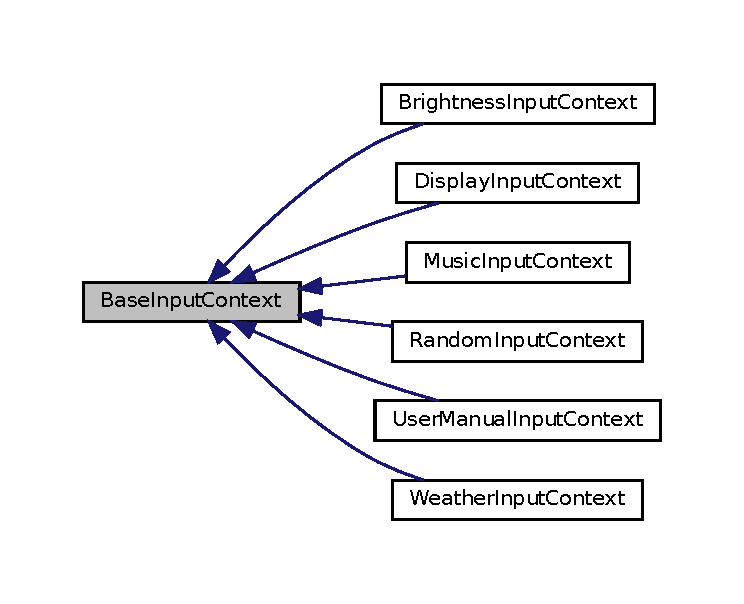
\includegraphics[width=350pt]{classBaseInputContext__inherit__graph}
\end{center}
\end{figure}


Collaboration diagram for Base\+Input\+Context\+:\nopagebreak
\begin{figure}[H]
\begin{center}
\leavevmode
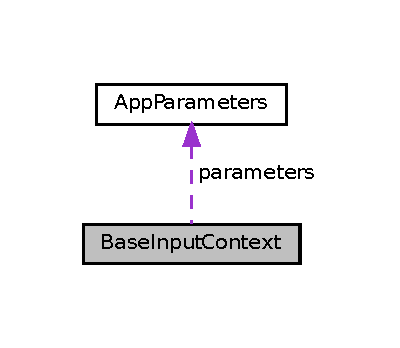
\includegraphics[width=192pt]{classBaseInputContext__coll__graph}
\end{center}
\end{figure}
\subsection*{Public Member Functions}
\begin{DoxyCompactItemize}
\item 
\mbox{\Hypertarget{classBaseInputContext_a7d8ee828f7bf345c42654d2d35c6b54b}\label{classBaseInputContext_a7d8ee828f7bf345c42654d2d35c6b54b}} 
{\bfseries Base\+Input\+Context} (\hyperlink{structAppParameters}{App\+Parameters} parameters, Input\+Types input\+\_\+type, bool active)
\item 
\mbox{\Hypertarget{classBaseInputContext_ab01c79b8298af7d22cca34d4cee4ed32}\label{classBaseInputContext_ab01c79b8298af7d22cca34d4cee4ed32}} 
{\bfseries Base\+Input\+Context} (\hyperlink{structAppParameters}{App\+Parameters} parameters, std\+::vector$<$ \hyperlink{classLEDContext}{L\+E\+D\+Context} $>$ \&\&led\+\_\+vector, Input\+Types input\+\_\+type, bool active)
\item 
\mbox{\Hypertarget{classBaseInputContext_a2a2342b849914cdad5e5fafb985198fe}\label{classBaseInputContext_a2a2342b849914cdad5e5fafb985198fe}} 
{\bfseries Base\+Input\+Context} (\hyperlink{classBaseInputContext}{Base\+Input\+Context} \&other)
\item 
\mbox{\Hypertarget{classBaseInputContext_a766e7f1c9c02069dec98870c84939d1e}\label{classBaseInputContext_a766e7f1c9c02069dec98870c84939d1e}} 
{\bfseries Base\+Input\+Context} (\hyperlink{classBaseInputContext}{Base\+Input\+Context} \&\&other)
\item 
\mbox{\Hypertarget{classBaseInputContext_a0c3354b22b4f98a9f29f0b8caff28593}\label{classBaseInputContext_a0c3354b22b4f98a9f29f0b8caff28593}} 
\hyperlink{classBaseInputContext}{Base\+Input\+Context} \& {\bfseries operator=} (\hyperlink{classBaseInputContext}{Base\+Input\+Context} \&other)
\item 
\mbox{\Hypertarget{classBaseInputContext_a63d4e572f54a59ee4fb045e066eaa132}\label{classBaseInputContext_a63d4e572f54a59ee4fb045e066eaa132}} 
\hyperlink{classBaseInputContext}{Base\+Input\+Context} \& {\bfseries operator=} (\hyperlink{classBaseInputContext}{Base\+Input\+Context} \&\&other)
\item 
\mbox{\Hypertarget{classBaseInputContext_a307ef6df7438b9ee911b190808b83e1f}\label{classBaseInputContext_a307ef6df7438b9ee911b190808b83e1f}} 
virtual std\+::tuple$<$ \hyperlink{structAppParameters}{App\+Parameters} \&, std\+::vector$<$ \hyperlink{classLEDContext}{L\+E\+D\+Context} $>$ \& $>$ {\bfseries Process} ()=0
\item 
\mbox{\Hypertarget{classBaseInputContext_a4caeb00d25a397c8e7d699cd12326d89}\label{classBaseInputContext_a4caeb00d25a397c8e7d699cd12326d89}} 
Input\+Types \hyperlink{classBaseInputContext_a4caeb00d25a397c8e7d699cd12326d89}{Get\+Input\+Type} () const noexcept
\begin{DoxyCompactList}\small\item\em Getter for the input context type. \end{DoxyCompactList}\item 
\mbox{\Hypertarget{classBaseInputContext_a990115f776002c595e3db3672301717d}\label{classBaseInputContext_a990115f776002c595e3db3672301717d}} 
std\+::vector$<$ \hyperlink{classLEDContext}{L\+E\+D\+Context} $>$ \& \hyperlink{classBaseInputContext_a990115f776002c595e3db3672301717d}{Get\+Led\+Vector} () noexcept
\begin{DoxyCompactList}\small\item\em Getter for the L\+ED vector. \end{DoxyCompactList}\item 
\mbox{\Hypertarget{classBaseInputContext_a3bbc32088faaf895d3cf1503bac2fb2f}\label{classBaseInputContext_a3bbc32088faaf895d3cf1503bac2fb2f}} 
\hyperlink{structAppParameters}{App\+Parameters} \& \hyperlink{classBaseInputContext_a3bbc32088faaf895d3cf1503bac2fb2f}{Get\+App\+Parameters} () noexcept
\begin{DoxyCompactList}\small\item\em Getter for the application parameters. \end{DoxyCompactList}\item 
\mbox{\Hypertarget{classBaseInputContext_ae6cc650533200b4f4c5f9c5dfdd19023}\label{classBaseInputContext_ae6cc650533200b4f4c5f9c5dfdd19023}} 
bool \hyperlink{classBaseInputContext_ae6cc650533200b4f4c5f9c5dfdd19023}{Is\+Active} () noexcept
\begin{DoxyCompactList}\small\item\em Getter for activity status. \end{DoxyCompactList}\item 
\mbox{\Hypertarget{classBaseInputContext_a3e3c544f5658e379a71228680a05b700}\label{classBaseInputContext_a3e3c544f5658e379a71228680a05b700}} 
void \hyperlink{classBaseInputContext_a3e3c544f5658e379a71228680a05b700}{Set\+App\+Parameters} (const \hyperlink{structAppParameters}{App\+Parameters} \&other\+\_\+parameters) noexcept
\begin{DoxyCompactList}\small\item\em Setter for application parameters. \end{DoxyCompactList}\item 
\mbox{\Hypertarget{classBaseInputContext_a31b87d03f2c28333e2b2a0bd746746d5}\label{classBaseInputContext_a31b87d03f2c28333e2b2a0bd746746d5}} 
void \hyperlink{classBaseInputContext_a31b87d03f2c28333e2b2a0bd746746d5}{Set\+Active} (bool is\+\_\+active) noexcept
\begin{DoxyCompactList}\small\item\em Setter for activity. \end{DoxyCompactList}\end{DoxyCompactItemize}
\subsection*{Protected Attributes}
\begin{DoxyCompactItemize}
\item 
\mbox{\Hypertarget{classBaseInputContext_a5fdbf0449f1db374d967fd5fe9f6d429}\label{classBaseInputContext_a5fdbf0449f1db374d967fd5fe9f6d429}} 
\hyperlink{structAppParameters}{App\+Parameters} {\bfseries parameters}
\item 
\mbox{\Hypertarget{classBaseInputContext_afbc4885e5ffea25ca766188ba74365dc}\label{classBaseInputContext_afbc4885e5ffea25ca766188ba74365dc}} 
std\+::vector$<$ \hyperlink{classLEDContext}{L\+E\+D\+Context} $>$ {\bfseries led\+\_\+vector}
\item 
\mbox{\Hypertarget{classBaseInputContext_ad8596def18b875e990a9097ecbc1f60f}\label{classBaseInputContext_ad8596def18b875e990a9097ecbc1f60f}} 
Input\+Types {\bfseries input\+\_\+type}
\item 
\mbox{\Hypertarget{classBaseInputContext_afc497040a6a6b44f3d753df6f0d70721}\label{classBaseInputContext_afc497040a6a6b44f3d753df6f0d70721}} 
bool {\bfseries active}
\end{DoxyCompactItemize}


\subsection{Detailed Description}
Base input context class for input processing. 

The documentation for this class was generated from the following file\+:\begin{DoxyCompactItemize}
\item 
inputcontext.\+hpp\end{DoxyCompactItemize}

\hypertarget{structBaseInputContextDeleter}{}\section{Base\+Input\+Context\+Deleter Struct Reference}
\label{structBaseInputContextDeleter}\index{Base\+Input\+Context\+Deleter@{Base\+Input\+Context\+Deleter}}


\hyperlink{classBaseInputContext}{Base\+Input\+Context} Templated Types.  




{\ttfamily \#include $<$device.\+hpp$>$}

\subsection*{Public Member Functions}
\begin{DoxyCompactItemize}
\item 
\mbox{\Hypertarget{structBaseInputContextDeleter_a4b9dd10f3b0edfc8d8f5691180088118}\label{structBaseInputContextDeleter_a4b9dd10f3b0edfc8d8f5691180088118}} 
void {\bfseries operator()} (\hyperlink{classBaseInputContext}{Base\+Input\+Context} $\ast$ptr)
\end{DoxyCompactItemize}


\subsection{Detailed Description}
\hyperlink{classBaseInputContext}{Base\+Input\+Context} Templated Types. 

The documentation for this struct was generated from the following file\+:\begin{DoxyCompactItemize}
\item 
device.\+hpp\end{DoxyCompactItemize}

\hypertarget{structBrightnessData}{}\section{Brightness\+Data Struct Reference}
\label{structBrightnessData}\index{Brightness\+Data@{Brightness\+Data}}


Data used for parsing the Brightness input.  




{\ttfamily \#include $<$inputcontext.\+hpp$>$}

\subsection*{Public Member Functions}
\begin{DoxyCompactItemize}
\item 
\mbox{\Hypertarget{structBrightnessData_a6ed915c802c53a45cbbe3157ddabe329}\label{structBrightnessData_a6ed915c802c53a45cbbe3157ddabe329}} 
{\bfseries Brightness\+Data} (std\+::vector$<$ unsigned char $>$ \&\&intensity\+Vector)
\end{DoxyCompactItemize}
\subsection*{Public Attributes}
\begin{DoxyCompactItemize}
\item 
\mbox{\Hypertarget{structBrightnessData_a84d67142636cadb91fd68e709fcdd0bf}\label{structBrightnessData_a84d67142636cadb91fd68e709fcdd0bf}} 
std\+::vector$<$ unsigned char $>$ {\bfseries intensity\+Vector}
\end{DoxyCompactItemize}


\subsection{Detailed Description}
Data used for parsing the Brightness input. 

The documentation for this struct was generated from the following file\+:\begin{DoxyCompactItemize}
\item 
inputcontext.\+hpp\end{DoxyCompactItemize}

\hypertarget{classBrightnessInputContext}{}\section{Brightness\+Input\+Context Class Reference}
\label{classBrightnessInputContext}\index{Brightness\+Input\+Context@{Brightness\+Input\+Context}}


Input context class for brightness input.  




{\ttfamily \#include $<$inputcontext.\+hpp$>$}



Inheritance diagram for Brightness\+Input\+Context\+:\nopagebreak
\begin{figure}[H]
\begin{center}
\leavevmode
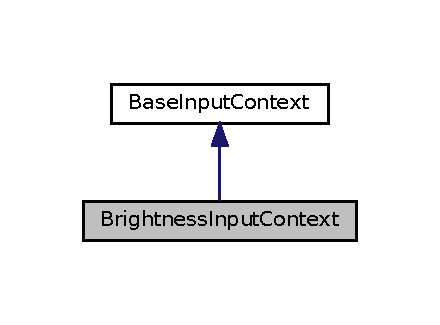
\includegraphics[width=211pt]{classBrightnessInputContext__inherit__graph}
\end{center}
\end{figure}


Collaboration diagram for Brightness\+Input\+Context\+:\nopagebreak
\begin{figure}[H]
\begin{center}
\leavevmode
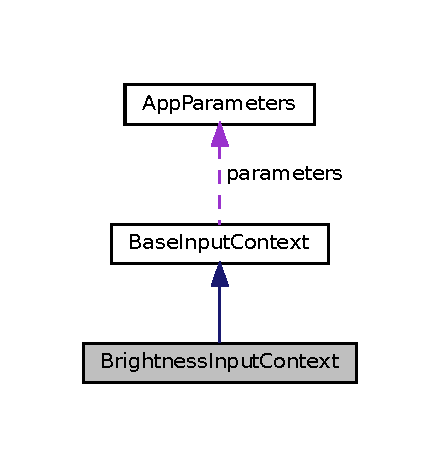
\includegraphics[width=211pt]{classBrightnessInputContext__coll__graph}
\end{center}
\end{figure}
\subsection*{Public Member Functions}
\begin{DoxyCompactItemize}
\item 
\mbox{\Hypertarget{classBrightnessInputContext_a152a2a28efc12b3f4c9461dcadfebfe7}\label{classBrightnessInputContext_a152a2a28efc12b3f4c9461dcadfebfe7}} 
{\bfseries Brightness\+Input\+Context} (\hyperlink{structAppParameters}{App\+Parameters} parameters, \hyperlink{structBrightnessData}{Brightness\+Data} brightness\+Data, bool active)
\item 
\mbox{\Hypertarget{classBrightnessInputContext_abed6703d2d678ba74efdd635b5e39104}\label{classBrightnessInputContext_abed6703d2d678ba74efdd635b5e39104}} 
std\+::tuple$<$ \hyperlink{structAppParameters}{App\+Parameters} \&, std\+::vector$<$ \hyperlink{classLEDContext}{L\+E\+D\+Context} $>$ \& $>$ {\bfseries Process} ()
\end{DoxyCompactItemize}
\subsection*{Additional Inherited Members}


\subsection{Detailed Description}
Input context class for brightness input. 

The documentation for this class was generated from the following file\+:\begin{DoxyCompactItemize}
\item 
inputcontext.\+hpp\end{DoxyCompactItemize}

\hypertarget{classDisplayInputContext}{}\section{Display\+Input\+Context Class Reference}
\label{classDisplayInputContext}\index{Display\+Input\+Context@{Display\+Input\+Context}}


Input context class for display input.  




{\ttfamily \#include $<$inputcontext.\+hpp$>$}



Inheritance diagram for Display\+Input\+Context\+:\nopagebreak
\begin{figure}[H]
\begin{center}
\leavevmode
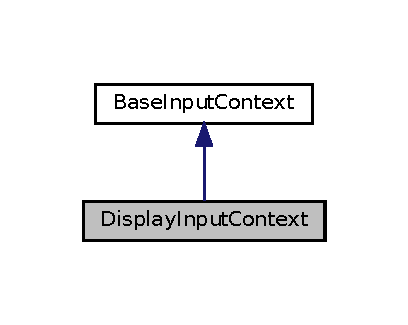
\includegraphics[width=196pt]{classDisplayInputContext__inherit__graph}
\end{center}
\end{figure}


Collaboration diagram for Display\+Input\+Context\+:\nopagebreak
\begin{figure}[H]
\begin{center}
\leavevmode
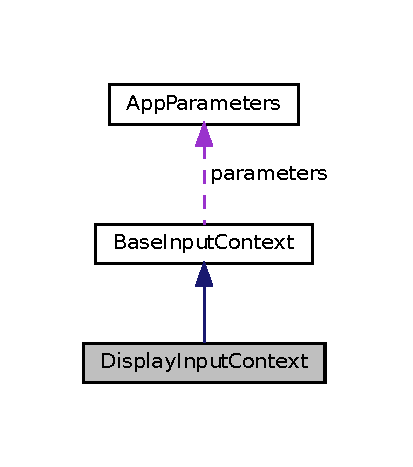
\includegraphics[width=198pt]{classDisplayInputContext__coll__graph}
\end{center}
\end{figure}
\subsection*{Public Member Functions}
\begin{DoxyCompactItemize}
\item 
\mbox{\Hypertarget{classDisplayInputContext_a5f5294995529afa72f09b86423a9cd8b}\label{classDisplayInputContext_a5f5294995529afa72f09b86423a9cd8b}} 
{\bfseries Display\+Input\+Context} (\hyperlink{structAppParameters}{App\+Parameters} parameters, std\+::vector$<$ \hyperlink{classLEDContext}{L\+E\+D\+Context} $>$ \&\&led\+\_\+vector, bool active)
\item 
\mbox{\Hypertarget{classDisplayInputContext_a311ae1f786cf44daa1945bd1bd22caa6}\label{classDisplayInputContext_a311ae1f786cf44daa1945bd1bd22caa6}} 
std\+::tuple$<$ \hyperlink{structAppParameters}{App\+Parameters} \&, std\+::vector$<$ \hyperlink{classLEDContext}{L\+E\+D\+Context} $>$ \& $>$ {\bfseries Process} ()
\end{DoxyCompactItemize}
\subsection*{Additional Inherited Members}


\subsection{Detailed Description}
Input context class for display input. 

The documentation for this class was generated from the following file\+:\begin{DoxyCompactItemize}
\item 
inputcontext.\+hpp\end{DoxyCompactItemize}

\hypertarget{classLEDContext}{}\section{L\+E\+D\+Context Class Reference}
\label{classLEDContext}\index{L\+E\+D\+Context@{L\+E\+D\+Context}}


L\+ED context class.  




{\ttfamily \#include $<$inputcontext.\+hpp$>$}

\subsection*{Public Member Functions}
\begin{DoxyCompactItemize}
\item 
\mbox{\Hypertarget{classLEDContext_a595fe959a611f75c6791ab40b1fb5dc0}\label{classLEDContext_a595fe959a611f75c6791ab40b1fb5dc0}} 
{\bfseries L\+E\+D\+Context} (unsigned char intensity, \hyperlink{structRGB}{R\+GB} rgb, bool visible)
\item 
\mbox{\Hypertarget{classLEDContext_a341d5800ea8fefee47326c9a78e909ec}\label{classLEDContext_a341d5800ea8fefee47326c9a78e909ec}} 
{\bfseries L\+E\+D\+Context} (const \hyperlink{classLEDContext}{L\+E\+D\+Context} \&led\+\_\+context)
\item 
\mbox{\Hypertarget{classLEDContext_a774a2e7001b38ed6bc74d721bc97715a}\label{classLEDContext_a774a2e7001b38ed6bc74d721bc97715a}} 
\hyperlink{structRGB}{R\+GB} {\bfseries get\+R\+GB} ()
\end{DoxyCompactItemize}


\subsection{Detailed Description}
L\+ED context class. 

The documentation for this class was generated from the following file\+:\begin{DoxyCompactItemize}
\item 
inputcontext.\+hpp\end{DoxyCompactItemize}

\hypertarget{classMqttSubscriber}{}\section{Mqtt\+Subscriber Class Reference}
\label{classMqttSubscriber}\index{Mqtt\+Subscriber@{Mqtt\+Subscriber}}
\subsection*{Public Member Functions}
\begin{DoxyCompactItemize}
\item 
\mbox{\Hypertarget{classMqttSubscriber_a1dc5293a63d0e9908ba6e2d067ad76d0}\label{classMqttSubscriber_a1dc5293a63d0e9908ba6e2d067ad76d0}} 
void {\bfseries Start\+Processing\+Inputs} ()
\end{DoxyCompactItemize}
\subsection*{Static Public Member Functions}
\begin{DoxyCompactItemize}
\item 
\mbox{\Hypertarget{classMqttSubscriber_a583fdadde54af3df974d6804a9686d4b}\label{classMqttSubscriber_a583fdadde54af3df974d6804a9686d4b}} 
static void {\bfseries publish\+To\+Third\+Party} (std\+::string message)
\item 
\mbox{\Hypertarget{classMqttSubscriber_a4bca80e48ea35bae160daf395da0ab9b}\label{classMqttSubscriber_a4bca80e48ea35bae160daf395da0ab9b}} 
static void {\bfseries Subscribe} (std\+::string message)
\end{DoxyCompactItemize}


The documentation for this class was generated from the following file\+:\begin{DoxyCompactItemize}
\item 
mqtt\+\_\+subscriber.\+hpp\end{DoxyCompactItemize}

\hypertarget{structMusicData}{}\section{Music\+Data Struct Reference}
\label{structMusicData}\index{Music\+Data@{Music\+Data}}


Data used for parsing the Music input.  




{\ttfamily \#include $<$inputcontext.\+hpp$>$}

\subsection*{Public Member Functions}
\begin{DoxyCompactItemize}
\item 
\mbox{\Hypertarget{structMusicData_aea401e148e5615e4eb1bd39154d9f0b4}\label{structMusicData_aea401e148e5615e4eb1bd39154d9f0b4}} 
{\bfseries Music\+Data} (std\+::vector$<$ double $>$ \&\&frequency\+Vector)
\end{DoxyCompactItemize}
\subsection*{Public Attributes}
\begin{DoxyCompactItemize}
\item 
\mbox{\Hypertarget{structMusicData_a172fa273494c06fd7c1ce0ebb7375264}\label{structMusicData_a172fa273494c06fd7c1ce0ebb7375264}} 
std\+::vector$<$ double $>$ {\bfseries frequency\+Vector}
\end{DoxyCompactItemize}


\subsection{Detailed Description}
Data used for parsing the Music input. 

The documentation for this struct was generated from the following file\+:\begin{DoxyCompactItemize}
\item 
inputcontext.\+hpp\end{DoxyCompactItemize}

\hypertarget{classMusicInputContext}{}\section{Music\+Input\+Context Class Reference}
\label{classMusicInputContext}\index{Music\+Input\+Context@{Music\+Input\+Context}}


Input context class for music input.  




{\ttfamily \#include $<$inputcontext.\+hpp$>$}



Inheritance diagram for Music\+Input\+Context\+:\nopagebreak
\begin{figure}[H]
\begin{center}
\leavevmode
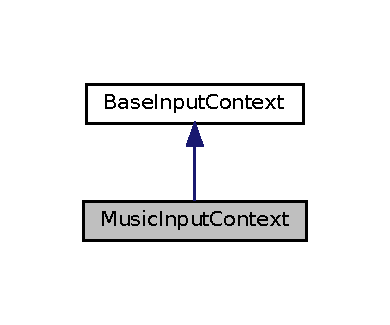
\includegraphics[width=187pt]{classMusicInputContext__inherit__graph}
\end{center}
\end{figure}


Collaboration diagram for Music\+Input\+Context\+:\nopagebreak
\begin{figure}[H]
\begin{center}
\leavevmode
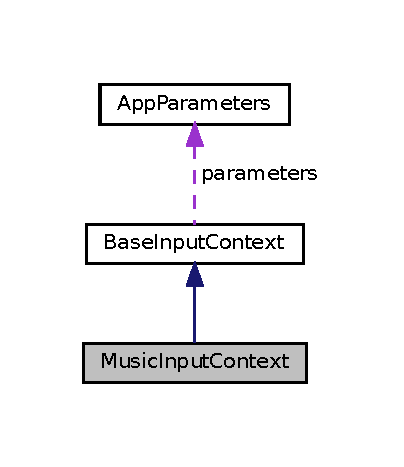
\includegraphics[width=194pt]{classMusicInputContext__coll__graph}
\end{center}
\end{figure}
\subsection*{Public Member Functions}
\begin{DoxyCompactItemize}
\item 
\mbox{\Hypertarget{classMusicInputContext_a3a684341715ba5a6db949843564d8bae}\label{classMusicInputContext_a3a684341715ba5a6db949843564d8bae}} 
{\bfseries Music\+Input\+Context} (\hyperlink{structAppParameters}{App\+Parameters} parameters, \hyperlink{structMusicData}{Music\+Data} music\+Data, bool active)
\item 
\mbox{\Hypertarget{classMusicInputContext_a3ebc756c72a1f7978f00ff10141291c8}\label{classMusicInputContext_a3ebc756c72a1f7978f00ff10141291c8}} 
std\+::tuple$<$ \hyperlink{structAppParameters}{App\+Parameters} \&, std\+::vector$<$ \hyperlink{classLEDContext}{L\+E\+D\+Context} $>$ \& $>$ {\bfseries Process} ()
\end{DoxyCompactItemize}
\subsection*{Additional Inherited Members}


\subsection{Detailed Description}
Input context class for music input. 

The documentation for this class was generated from the following file\+:\begin{DoxyCompactItemize}
\item 
inputcontext.\+hpp\end{DoxyCompactItemize}

\hypertarget{classRandomInputContext}{}\section{Random\+Input\+Context Class Reference}
\label{classRandomInputContext}\index{Random\+Input\+Context@{Random\+Input\+Context}}


Input context class for random input.  




{\ttfamily \#include $<$inputcontext.\+hpp$>$}



Inheritance diagram for Random\+Input\+Context\+:\nopagebreak
\begin{figure}[H]
\begin{center}
\leavevmode
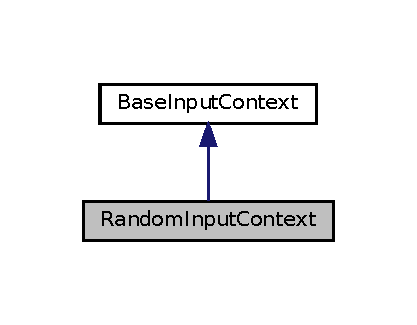
\includegraphics[width=200pt]{classRandomInputContext__inherit__graph}
\end{center}
\end{figure}


Collaboration diagram for Random\+Input\+Context\+:\nopagebreak
\begin{figure}[H]
\begin{center}
\leavevmode
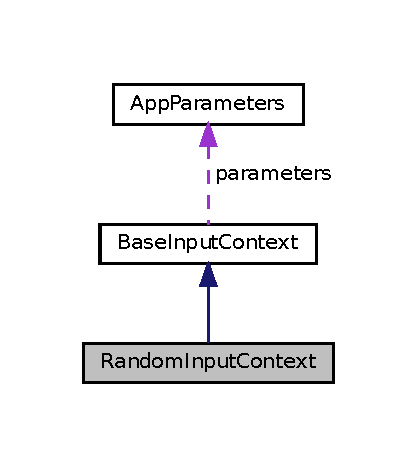
\includegraphics[width=200pt]{classRandomInputContext__coll__graph}
\end{center}
\end{figure}
\subsection*{Public Member Functions}
\begin{DoxyCompactItemize}
\item 
\mbox{\Hypertarget{classRandomInputContext_ab2747e77324ec4e5dec7c19bbe8711bf}\label{classRandomInputContext_ab2747e77324ec4e5dec7c19bbe8711bf}} 
{\bfseries Random\+Input\+Context} (\hyperlink{structAppParameters}{App\+Parameters} parameters, bool active)
\item 
\mbox{\Hypertarget{classRandomInputContext_a19ab176510befce3e8f029cd946081f6}\label{classRandomInputContext_a19ab176510befce3e8f029cd946081f6}} 
std\+::tuple$<$ \hyperlink{structAppParameters}{App\+Parameters} \&, std\+::vector$<$ \hyperlink{classLEDContext}{L\+E\+D\+Context} $>$ \& $>$ {\bfseries Process} ()
\end{DoxyCompactItemize}
\subsection*{Additional Inherited Members}


\subsection{Detailed Description}
Input context class for random input. 

The documentation for this class was generated from the following file\+:\begin{DoxyCompactItemize}
\item 
inputcontext.\+hpp\end{DoxyCompactItemize}

\hypertarget{structRGB}{}\section{R\+GB Struct Reference}
\label{structRGB}\index{R\+GB@{R\+GB}}


\hyperlink{structRGB}{R\+GB} data structure.  




{\ttfamily \#include $<$inputcontext.\+hpp$>$}

\subsection*{Public Member Functions}
\begin{DoxyCompactItemize}
\item 
\mbox{\Hypertarget{structRGB_ae5c6f8e87d889304b591d841ed635ec9}\label{structRGB_ae5c6f8e87d889304b591d841ed635ec9}} 
{\bfseries R\+GB} (unsigned char \+\_\+r, unsigned char \+\_\+g, unsigned char \+\_\+b)
\item 
\mbox{\Hypertarget{structRGB_adf1461c8cdffc074a2e019dc9d1f3bc1}\label{structRGB_adf1461c8cdffc074a2e019dc9d1f3bc1}} 
{\bfseries R\+GB} (const \hyperlink{structRGB}{R\+GB} \&rgb)
\item 
\mbox{\Hypertarget{structRGB_a4a5e452c99048fbf1c71e2983794a982}\label{structRGB_a4a5e452c99048fbf1c71e2983794a982}} 
unsigned char {\bfseries get\+Red} ()
\item 
\mbox{\Hypertarget{structRGB_a1744e7db1a6f3f7aa527c7c892ac422b}\label{structRGB_a1744e7db1a6f3f7aa527c7c892ac422b}} 
unsigned char {\bfseries get\+Green} ()
\item 
\mbox{\Hypertarget{structRGB_a641b32101c60fc25ef1f91be5ae0264c}\label{structRGB_a641b32101c60fc25ef1f91be5ae0264c}} 
unsigned char {\bfseries get\+Blue} ()
\end{DoxyCompactItemize}
\subsection*{Public Attributes}
\begin{DoxyCompactItemize}
\item 
\mbox{\Hypertarget{structRGB_a8ea970fcd312802ef238733b1c9ed63d}\label{structRGB_a8ea970fcd312802ef238733b1c9ed63d}} 
unsigned char {\bfseries r}
\item 
\mbox{\Hypertarget{structRGB_a3595e9a2ed44c815153aff4e84e2d97c}\label{structRGB_a3595e9a2ed44c815153aff4e84e2d97c}} 
unsigned char {\bfseries g}
\item 
\mbox{\Hypertarget{structRGB_ab2a3ac761d61594e2c51d65347a74017}\label{structRGB_ab2a3ac761d61594e2c51d65347a74017}} 
unsigned char {\bfseries b}
\end{DoxyCompactItemize}


\subsection{Detailed Description}
\hyperlink{structRGB}{R\+GB} data structure. 

The documentation for this struct was generated from the following file\+:\begin{DoxyCompactItemize}
\item 
inputcontext.\+hpp\end{DoxyCompactItemize}

\hypertarget{structUserManualData}{}\section{User\+Manual\+Data Struct Reference}
\label{structUserManualData}\index{User\+Manual\+Data@{User\+Manual\+Data}}


Data used for parsing the User\+Manual input.  




{\ttfamily \#include $<$inputcontext.\+hpp$>$}



Collaboration diagram for User\+Manual\+Data\+:\nopagebreak
\begin{figure}[H]
\begin{center}
\leavevmode
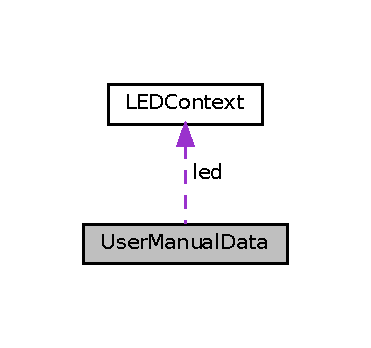
\includegraphics[width=178pt]{structUserManualData__coll__graph}
\end{center}
\end{figure}
\subsection*{Public Member Functions}
\begin{DoxyCompactItemize}
\item 
\mbox{\Hypertarget{structUserManualData_a598240dc298cc519dffc1a73c9c911cb}\label{structUserManualData_a598240dc298cc519dffc1a73c9c911cb}} 
{\bfseries User\+Manual\+Data} (\hyperlink{classLEDContext}{L\+E\+D\+Context} led)
\end{DoxyCompactItemize}
\subsection*{Public Attributes}
\begin{DoxyCompactItemize}
\item 
\mbox{\Hypertarget{structUserManualData_aec74f70aeef43227b6b1a494333687df}\label{structUserManualData_aec74f70aeef43227b6b1a494333687df}} 
\hyperlink{classLEDContext}{L\+E\+D\+Context} {\bfseries led}
\end{DoxyCompactItemize}


\subsection{Detailed Description}
Data used for parsing the User\+Manual input. 

The documentation for this struct was generated from the following file\+:\begin{DoxyCompactItemize}
\item 
inputcontext.\+hpp\end{DoxyCompactItemize}

\hypertarget{classUserManualInputContext}{}\section{User\+Manual\+Input\+Context Class Reference}
\label{classUserManualInputContext}\index{User\+Manual\+Input\+Context@{User\+Manual\+Input\+Context}}


Input context class for manual user input.  




{\ttfamily \#include $<$inputcontext.\+hpp$>$}



Inheritance diagram for User\+Manual\+Input\+Context\+:\nopagebreak
\begin{figure}[H]
\begin{center}
\leavevmode
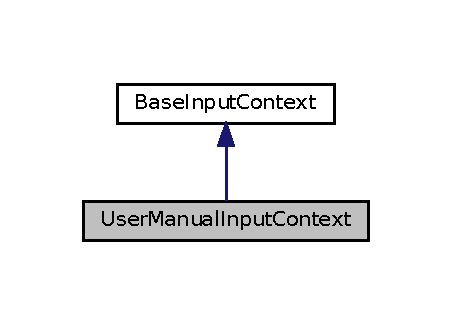
\includegraphics[width=217pt]{classUserManualInputContext__inherit__graph}
\end{center}
\end{figure}


Collaboration diagram for User\+Manual\+Input\+Context\+:\nopagebreak
\begin{figure}[H]
\begin{center}
\leavevmode
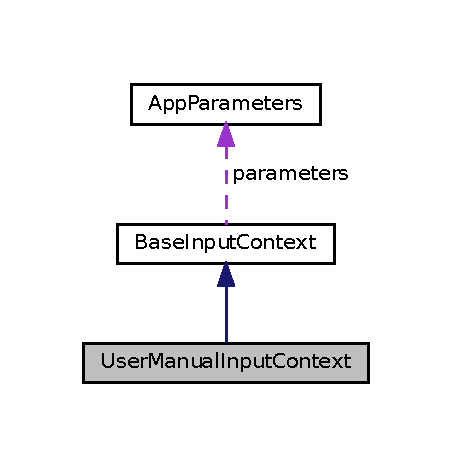
\includegraphics[width=217pt]{classUserManualInputContext__coll__graph}
\end{center}
\end{figure}
\subsection*{Public Member Functions}
\begin{DoxyCompactItemize}
\item 
\mbox{\Hypertarget{classUserManualInputContext_a3ee58341cb01d323935413b9b5cb80f2}\label{classUserManualInputContext_a3ee58341cb01d323935413b9b5cb80f2}} 
{\bfseries User\+Manual\+Input\+Context} (\hyperlink{structAppParameters}{App\+Parameters} parameters, \hyperlink{structUserManualData}{User\+Manual\+Data} user\+Manual\+Data, bool active)
\item 
\mbox{\Hypertarget{classUserManualInputContext_aac7943547f0441ae5f2391985650b393}\label{classUserManualInputContext_aac7943547f0441ae5f2391985650b393}} 
std\+::tuple$<$ \hyperlink{structAppParameters}{App\+Parameters} \&, std\+::vector$<$ \hyperlink{classLEDContext}{L\+E\+D\+Context} $>$ \& $>$ {\bfseries Process} ()
\end{DoxyCompactItemize}
\subsection*{Additional Inherited Members}


\subsection{Detailed Description}
Input context class for manual user input. 

The documentation for this class was generated from the following file\+:\begin{DoxyCompactItemize}
\item 
inputcontext.\+hpp\end{DoxyCompactItemize}

\hypertarget{structWeatherData}{}\section{Weather\+Data Struct Reference}
\label{structWeatherData}\index{Weather\+Data@{Weather\+Data}}


Data used for parsing the Weather input.  




{\ttfamily \#include $<$inputcontext.\+hpp$>$}

\subsection*{Public Member Functions}
\begin{DoxyCompactItemize}
\item 
\mbox{\Hypertarget{structWeatherData_a9775ece73c6ac6082cf7edba50e4bd47}\label{structWeatherData_a9775ece73c6ac6082cf7edba50e4bd47}} 
{\bfseries Weather\+Data} (float temperature)
\end{DoxyCompactItemize}
\subsection*{Public Attributes}
\begin{DoxyCompactItemize}
\item 
\mbox{\Hypertarget{structWeatherData_a9b81dcf968ae2f54d349ffc3101b6fdd}\label{structWeatherData_a9b81dcf968ae2f54d349ffc3101b6fdd}} 
float {\bfseries temperature}
\end{DoxyCompactItemize}


\subsection{Detailed Description}
Data used for parsing the Weather input. 

The documentation for this struct was generated from the following file\+:\begin{DoxyCompactItemize}
\item 
inputcontext.\+hpp\end{DoxyCompactItemize}

\hypertarget{classWeatherInputContext}{}\section{Weather\+Input\+Context Class Reference}
\label{classWeatherInputContext}\index{Weather\+Input\+Context@{Weather\+Input\+Context}}


Input context class for weather input.  




{\ttfamily \#include $<$inputcontext.\+hpp$>$}



Inheritance diagram for Weather\+Input\+Context\+:\nopagebreak
\begin{figure}[H]
\begin{center}
\leavevmode
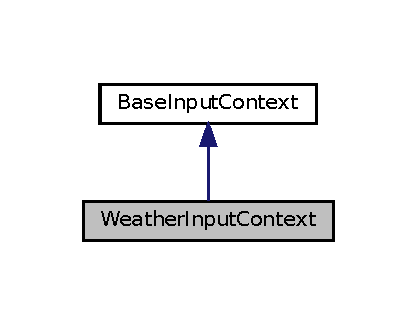
\includegraphics[width=200pt]{classWeatherInputContext__inherit__graph}
\end{center}
\end{figure}


Collaboration diagram for Weather\+Input\+Context\+:\nopagebreak
\begin{figure}[H]
\begin{center}
\leavevmode
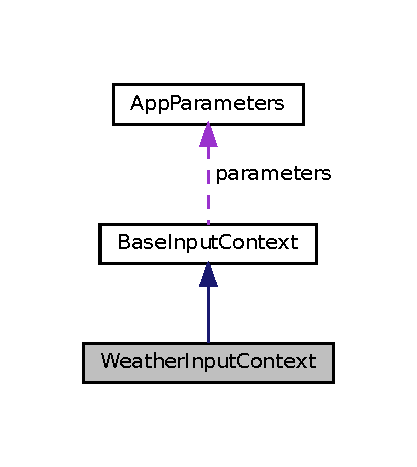
\includegraphics[width=200pt]{classWeatherInputContext__coll__graph}
\end{center}
\end{figure}
\subsection*{Public Member Functions}
\begin{DoxyCompactItemize}
\item 
\mbox{\Hypertarget{classWeatherInputContext_aed3db9e07794a5a475137b36d1356209}\label{classWeatherInputContext_aed3db9e07794a5a475137b36d1356209}} 
{\bfseries Weather\+Input\+Context} (\hyperlink{structAppParameters}{App\+Parameters} parameters, \hyperlink{structWeatherData}{Weather\+Data} weather\+Data, bool active)
\item 
\mbox{\Hypertarget{classWeatherInputContext_ad25230f426a5f5cacb527aea75e6ccc6}\label{classWeatherInputContext_ad25230f426a5f5cacb527aea75e6ccc6}} 
std\+::tuple$<$ \hyperlink{structAppParameters}{App\+Parameters} \&, std\+::vector$<$ \hyperlink{classLEDContext}{L\+E\+D\+Context} $>$ \& $>$ {\bfseries Process} ()
\end{DoxyCompactItemize}
\subsection*{Additional Inherited Members}


\subsection{Detailed Description}
Input context class for weather input. 

The documentation for this class was generated from the following file\+:\begin{DoxyCompactItemize}
\item 
inputcontext.\+hpp\end{DoxyCompactItemize}

\chapter{File Documentation}
\hypertarget{main_8cpp}{}\section{main.\+cpp File Reference}
\label{main_8cpp}\index{main.\+cpp@{main.\+cpp}}


Driver program for the project, exposes an H\+T\+TP server on port 8080 to handle A\+PI requests.  


{\ttfamily \#include $<$set$>$}\newline
{\ttfamily \#include $<$cstdio$>$}\newline
{\ttfamily \#include $<$string$>$}\newline
{\ttfamily \#include $<$stdexcept$>$}\newline
{\ttfamily \#include \char`\"{}device.\+hpp\char`\"{}}\newline
{\ttfamily \#include \char`\"{}mqtt\+\_\+subscriber.\+hpp\char`\"{}}\newline
Include dependency graph for main.\+cpp\+:
\nopagebreak
\begin{figure}[H]
\begin{center}
\leavevmode
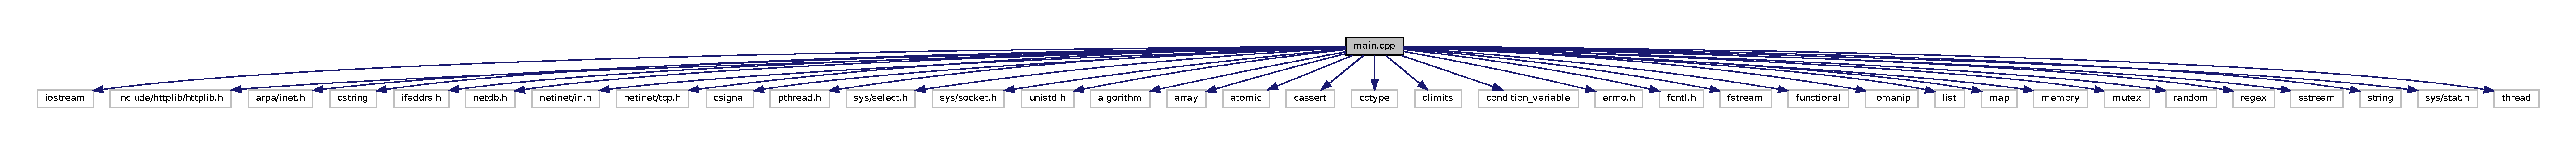
\includegraphics[width=350pt]{main_8cpp__incl}
\end{center}
\end{figure}
\subsection*{Macros}
\begin{DoxyCompactItemize}
\item 
\mbox{\Hypertarget{main_8cpp_a70bb99d4d6c2e1a35c26a6c84222be7f}\label{main_8cpp_a70bb99d4d6c2e1a35c26a6c84222be7f}} 
\#define {\bfseries I\+N\+P\+U\+T\+\_\+\+K\+EY}~\char`\"{}input\char`\"{}
\item 
\mbox{\Hypertarget{main_8cpp_aaf1329031adc4fd484b6edc8abfd7434}\label{main_8cpp_aaf1329031adc4fd484b6edc8abfd7434}} 
\#define {\bfseries I\+N\+P\+U\+T\+\_\+\+T\+Y\+P\+E\+\_\+\+K\+EY}~\char`\"{}input\+\_\+type\char`\"{}
\item 
\mbox{\Hypertarget{main_8cpp_af2685dfc271d06adb84a0d94a31d0de3}\label{main_8cpp_af2685dfc271d06adb84a0d94a31d0de3}} 
\#define {\bfseries I\+N\+P\+U\+T\+\_\+\+S\+E\+T\+T\+I\+N\+G\+S\+\_\+\+K\+EY}~\char`\"{}input\+\_\+settings\char`\"{}
\item 
\mbox{\Hypertarget{main_8cpp_a35c11f02aa6db89430334483bd425831}\label{main_8cpp_a35c11f02aa6db89430334483bd425831}} 
\#define {\bfseries O\+U\+T\+P\+U\+T\+\_\+\+E\+R\+R\+O\+R\+\_\+\+K\+EY}~\char`\"{}error\char`\"{}
\item 
\mbox{\Hypertarget{main_8cpp_a6bb3b62d951dfd91bb84d00c6d4580ea}\label{main_8cpp_a6bb3b62d951dfd91bb84d00c6d4580ea}} 
\#define {\bfseries O\+U\+T\+P\+U\+T\+\_\+\+V\+A\+L\+I\+D\+\_\+\+K\+EY}~\char`\"{}valid\+\_\+request\char`\"{}
\item 
\mbox{\Hypertarget{main_8cpp_a3cdc10e08bf545f186ce9ddc0f347dc0}\label{main_8cpp_a3cdc10e08bf545f186ce9ddc0f347dc0}} 
\#define {\bfseries I\+N\+V\+A\+L\+I\+D\+\_\+\+R\+E\+Q\+U\+E\+S\+T\+\_\+\+B\+O\+DY}~\char`\"{}invalid\+\_\+request\char`\"{}
\item 
\mbox{\Hypertarget{main_8cpp_a20ec364faebf30a95ab7d9cad53f1f24}\label{main_8cpp_a20ec364faebf30a95ab7d9cad53f1f24}} 
\#define {\bfseries B\+A\+D\+\_\+\+R\+E\+Q\+U\+E\+S\+T\+\_\+\+J\+S\+ON}~\char`\"{}request format isn\textquotesingle{}t correct\char`\"{}
\end{DoxyCompactItemize}
\subsection*{Functions}
\begin{DoxyCompactItemize}
\item 
int \hyperlink{main_8cpp_a840291bc02cba5474a4cb46a9b9566fe}{main} (void)
\begin{DoxyCompactList}\small\item\em Main driver function of the program, runs an H\+T\+TP server on port 8080 to process incoming requests (blocking!) \end{DoxyCompactList}\end{DoxyCompactItemize}
\subsection*{Variables}
\begin{DoxyCompactItemize}
\item 
const std\+::set$<$ std\+::string $>$ {\bfseries Input\+Type}
\end{DoxyCompactItemize}


\subsection{Detailed Description}
Driver program for the project, exposes an H\+T\+TP server on port 8080 to handle A\+PI requests. 



\subsection{Function Documentation}
\mbox{\Hypertarget{main_8cpp_a840291bc02cba5474a4cb46a9b9566fe}\label{main_8cpp_a840291bc02cba5474a4cb46a9b9566fe}} 
\index{main.\+cpp@{main.\+cpp}!main@{main}}
\index{main@{main}!main.\+cpp@{main.\+cpp}}
\subsubsection{\texorpdfstring{main()}{main()}}
{\footnotesize\ttfamily int main (\begin{DoxyParamCaption}\item[{void}]{ }\end{DoxyParamCaption})}



Main driver function of the program, runs an H\+T\+TP server on port 8080 to process incoming requests (blocking!) 

\begin{DoxyReturn}{Returns}
int -\/ status code 
\end{DoxyReturn}


\subsection{Variable Documentation}
\mbox{\Hypertarget{main_8cpp_a0320ad1b70d522baab095239e6454546}\label{main_8cpp_a0320ad1b70d522baab095239e6454546}} 
\index{main.\+cpp@{main.\+cpp}!Input\+Type@{Input\+Type}}
\index{Input\+Type@{Input\+Type}!main.\+cpp@{main.\+cpp}}
\subsubsection{\texorpdfstring{Input\+Type}{InputType}}
{\footnotesize\ttfamily const std\+::set$<$std\+::string$>$ Input\+Type}

{\bfseries Initial value\+:}
\begin{DoxyCode}
= \{
    \textcolor{stringliteral}{"UserManualInput"},
    \textcolor{stringliteral}{"DisplayInput"},
    \textcolor{stringliteral}{"MusicInput"},
    \textcolor{stringliteral}{"WeatherInput"},
    \textcolor{stringliteral}{"BrightnessInput"},
    \textcolor{stringliteral}{"RandomInput"}\}
\end{DoxyCode}

%--- End generated contents ---

% Index
\backmatter
\newpage
\phantomsection
\clearemptydoublepage
\addcontentsline{toc}{chapter}{Index}
\printindex

\end{document}
